\documentclass[Bachelorarbeit.tex]{subfiles}
\begin{document}
\chapter{Konzeption}
\label{chap:entwicklung}
Nachdem im letzten Kapitel die allgemeinen Analysen durchgeführt wurden soll im Verlauf dieses Kapitels, die Planung für den Prototypen abgeschlossen werden.
Für diesen Zweck wird, aufbauend auf den Ergebnissen der bisherigen Kapitel, ein Konzept erstellt welches im folgenden Kapitel (\nameref{chap:implementierung}) umgesetzt wird. \\
\\
Zusätzlich zu den bisherigen Analysen findet sich in diesem Kapitel noch die Dokumentation der durchgeführten \nameref{chap:analyse:sec:interviews}.
Diese \nameref{chap:analyse:sec:interviews} wurden durchgeführt um zu analysieren auf welche Art und Weise  Domänenexpert\_innen arbeiten.
Zum einen soll herausgefunden werden, wo sich aktuell Flaschenhälse, in ihren Workflows befinden und zum anderen, was sie für Wünsche und Anforderungen an ihre Planungswerkzeuge stellen.\\
\\
Anschließend wird, auf den Personen aus den \nameref{chap:analyse:sec:interviews} aufbauend eine \nameref{persona} erstellt.
Dies porträtieren eine fiktive Person aus der Zielgruppe und soll als Avatar die Entwicklung unterstützen um den Prototypen möglichst zielgerichtet auszuarbeiten.
\\
\\
Designentwurf

\section{Interviews}
\label{chap:analyse:sec:interviews}
Dieser Teil beschäftigt sich mit der Fragestellung, wie Personen ihre Außendienstlichen Tätigkeiten organisieren, welchen Herausforderungen sie im beruflichen Alltag gegenüberstehen und welche Verbesserungen sie sich wünschen. 
Für diesen Zweck sollen Interviews und Hand-ons  geführt werden, die sich an einem, eigens dafür erstellten, Leitfaden orientieren (siehe Anhang: \nameref{anhang:leitfaden_interviews}). 
Das Ziel dieser Interviews besteht darin, ein besseres Gefühl für den Ist-Zustand zu bekommen und Anhand dieser Erkenntnisse die möglichen Defizite zu analysieren.
Des weiteren bietet der Ansatz die Möglichkeit, Verbesserungswünsche und Ideen von Personen aus d1er Domäne zu erhalten ohne das sie zuvor durch den Blick aus technischer Sicht verfälscht wurden.

\subsection{Ausarbeitung des Leitfadens}

Als erster Schritt soll ein Leitfaden für die Interviews definiert werden. 
Dieser soll zum einen als Gedankenstütze für die Interviews dienen und zum anderen, in Form eines roter Fadens, zu einem strukturierten Ablauf führen.
Das Ziel der Interviews liegt darin, ein besseres Verständnis zu erlangen wie die einzelnen Personen arbeiten und mit welchen Mitteln.
Diese Informationen bilden eine wichtige Grundlage um bestehende Probleme und Stolpersteine zu im aktuellen Workflow zu identifizieren und bei der Realisierung des Prototypen zu vermeiden. 
Des weiteren bilden die Interviews einen wichtigen Einblick in die Domäne, anhand derer eine Nutzer\_innen zentriert Lösung, so nah wie möglich an der Realität entwickelt werden soll.\\
\\
Grundsätzlich sollten allgemeine Informationen zum Interview festgehalten werden wie die Dauer und das Datum des Interviews.
Bezüglich der Person sind das Tätigkeit im Unternehmen, die Verantwortung bei der Planung und die Art der Beschäftigung (angestellt oder selbstständig) interessant.
Des weiteren spielt die Größe, das Betätigungsfeld und das Einzugsgebiete des Unternehmens eine Rolle für die Befragung.
Um eine bessere Strukturierung der Informationen zu erhalten wird zu erst der Standartablauf erfragt. 
Anschließend wird geklärt welche Sonderfälle auftreten können und wie diese jeweils gehandhabt werden.
Den Abschluss der Befragung bildet eine Selbstbeurteilung des Workflows. 
Dieser ist zum einen in Probleme und zum anderen in Wünsche unterteilt.
Bei dem ersten Punkt wird explizit nachgefragt welche Probleme oder Engstellen die Probanden im Alltag festgestellt haben.
Während bei dem zweiten Punkt nach den Wünschen beziehungsweise Sinnvollen Ergänzungen gefragt werden die sie sich selbst überlegt haben. 
Die finale Version des Leitfadens kann im Anhang eingesehen werden (\nameref{anhang:leitfaden_interviews}). 







\section{Ergebnisse der Interviews}
Bei den Personen handelt es sich um drei verschiedene Individuen die in drei verschiedenen Berufen in drei verschiedenen Firmen arbeiten und für ihren Alltag die unterschiedlichsten Systeme und Medien verwenden. 
Dabei sind alle befragten Personen seit mindestens zwei Jahren in ihrer Funktion tätig und sind für die Planung ihrer Routen selbst verantwortlich.
\\
\\
Für eine bessere Übersicht, ist die Ausarbeitung der Ergebnisse in die drei Gruppen:
\nameref{UebersichtDerInterviews}, \nameref{subsubsec:Ergebnisse der Interviews:gemeinsamkeiten} und \nameref{AnalyseInterviews} unterteilt. 


\subsection{Übersicht der Interviews}
\label{UebersichtDerInterviews}
\paragraph*{Übersicht - \nameref{anhang:interview1}} 

Die Person arbeitet für einen nationalen Konzern im Bereich Dienstleistung in der Arbeitskräftevermittlung. 
Der Einzugsbereich umfasst ausschließlich das Land Vorarlberg, Österreich.
Während die Kontaktdaten über das hauseigene \ac{ERP} gepflegt und gesucht werden, wird die Terminplanung und -Verwaltung größtenteils mithilfe eines Taschenkalenders abgewickelt.
Dabei wird im voraus für jede Kalenderwoche eine Region definiert. 
Für die gewählte Kalenderwoche werden mit Kunden in der entsprechenden Region Termine vereinbart.\\
\\
Folgende Abbildung (Abb.: \ref{fig:ProblemeInterview1} \nameref{fig:ProblemeInterview1}) zeigt die Verteilung der Probleme welche im ersten Interview genannt wurden. 
Diese sind \nameref{p1}, \nameref{p4} und \nameref{p6} (Siehe Abschnitt \ref{subsubsec:Ergebnisse der Interviews:probleme} \nameref{subsubsec:Ergebnisse der Interviews:probleme} für weitere Informationen).

\begin{figure}[h]
\centering
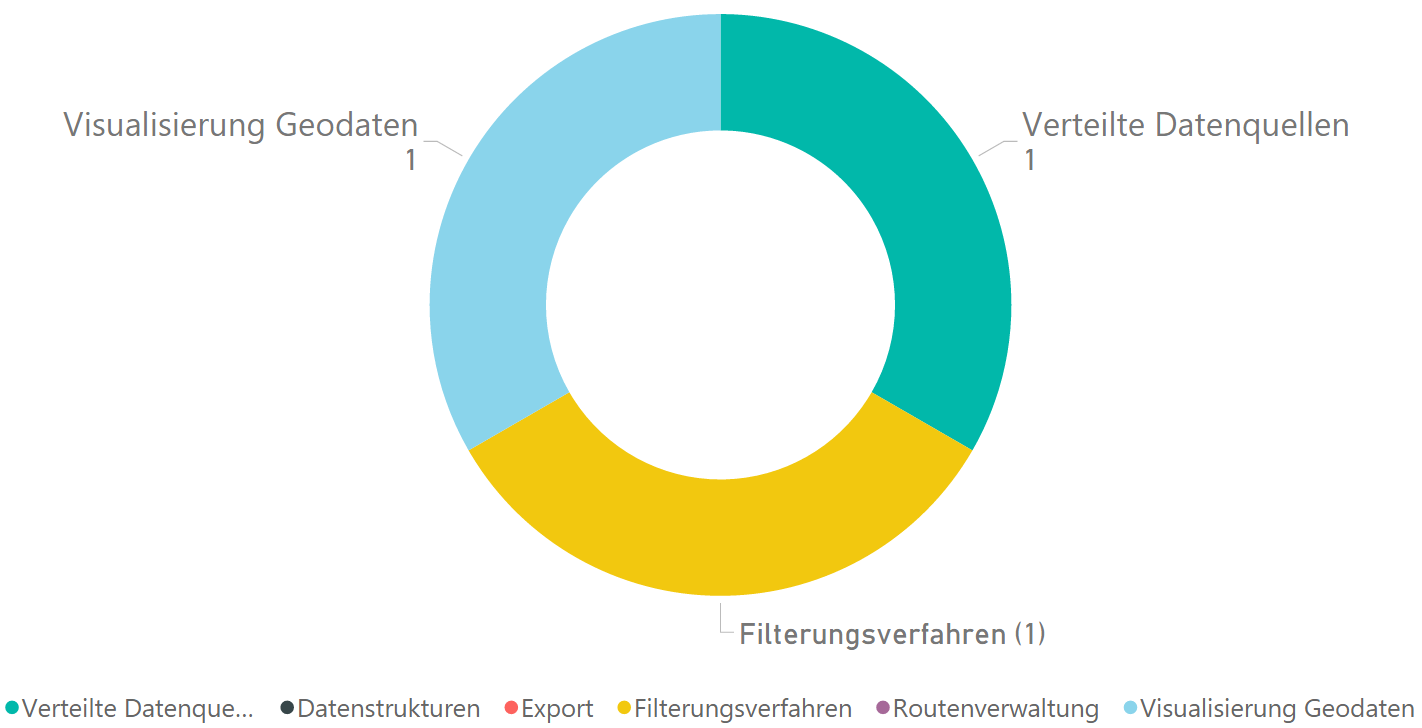
\includegraphics[width=1\linewidth]{img/Interviews/ProblemeInterview1}
\caption[Probleme Interview I]{Übersicht der genannten Probleme in Interview I (Quelle: eigene Ausarbeitung)}
\label{fig:ProblemeInterview1}
\end{figure}



\paragraph*{Übersicht - \nameref{anhang:interview2}}
Bei dem zweiten Interview handelt es sich um eine Person die zum einen für die Leitung der Firma sowie den Außendienst verantwortlich ist.
Der Tätigkeitsbereich des \ac{KMU}, mit Firmensitz in Wien, bezieht sich auf den Vertrieb von Hifi-Geräten für den professionellen Einsatz in Tonstudios.
Neben Österreich und dem EU-Raum gehört auch Russland zu dem Zuständigkeitsbereich des Unternehmens.
Dabei werden Außendienstrouten nach Bedarf geplannt.
Für diesen Zweck wird im ersten Schritt eine Route definiert. 
Anschließend werden, auf Basis der Route, die relevanten Bezirke rausgesucht.
Anhand einer Postleitzahlenkarte werden, in mehreren Schritten, die Postleitzahlen analysiert welche auf der Route liegen.
Diese Postleitzahlen dienen als Kriterium für den Filtervorgang im Kundenverzeichnis auf Basis dessen Schlussendlich die Kunden ausgesucht werden.\\
\\
Folgende Abbildung (Abb.: \ref{fig:ProblemeInterview2} \nameref{fig:ProblemeInterview2}) zeigt die Verteilung der Probleme welche im zweiten Interview genannt wurden. 
Diese sind \nameref{p1}, \nameref{p2}, \nameref{p3}, \nameref{p4}, \nameref{p5} und \nameref{p6} (Siehe Abschnitt \ref{subsubsec:Ergebnisse der Interviews:probleme} \nameref{subsubsec:Ergebnisse der Interviews:probleme} für weitere Informationen).
\begin{figure}[h]
\centering
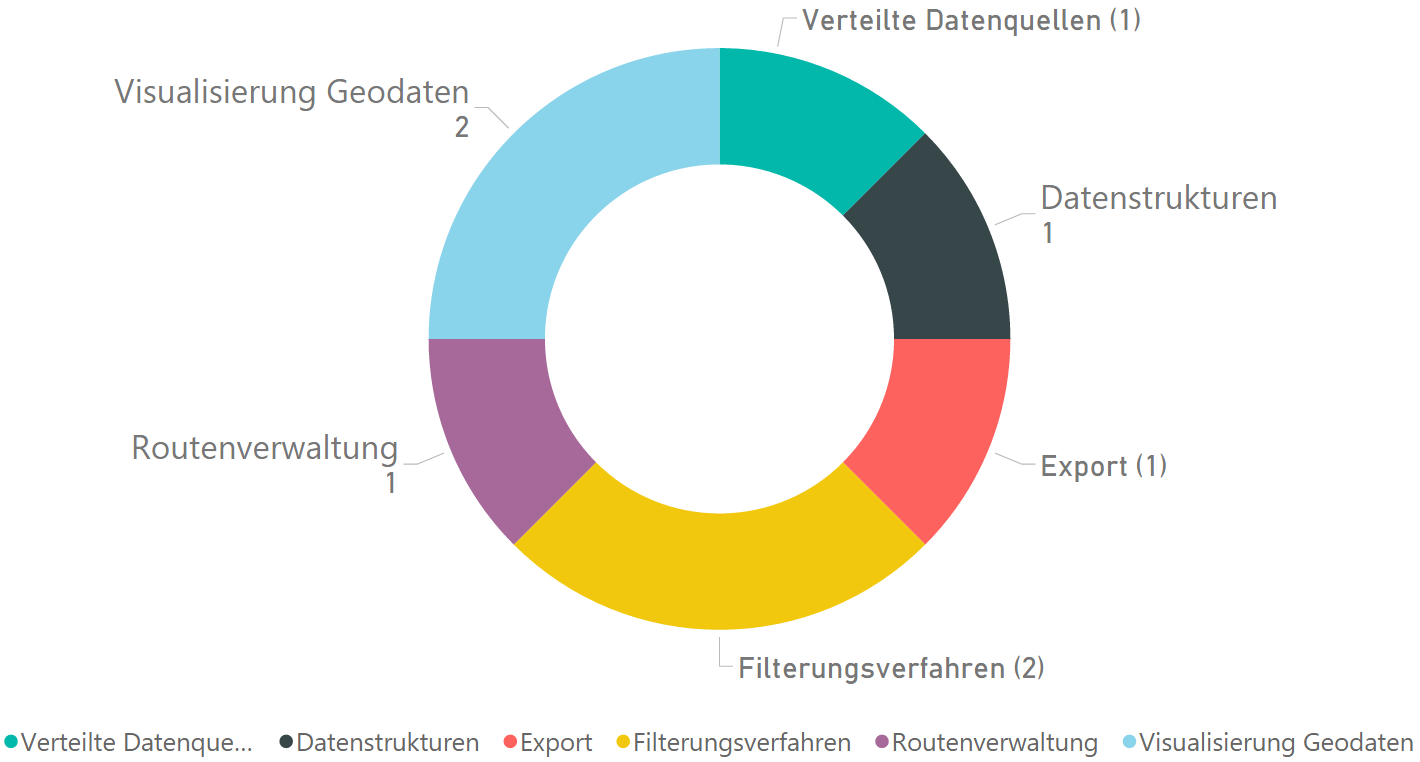
\includegraphics[width=1\linewidth]{img/Interviews/ProblemeInterview2}
\caption[Probleme in Interview II]{Übersicht der genannten Probleme in Interview II (Quelle: eigene Ausarbeitung)}
\label{fig:ProblemeInterview2}
\end{figure}


\paragraph*{Übersicht - \nameref{anhang:interview3}}
Bei dem letzten Interview handelt es sich um eine Person welche eine Anstellung in den Bereichen des Key Account Management sowie Projektleitung in einem \ac{KMU} inne hat.
Bei dem Unternehmen selbst handelt es sich um eine Werbeagentur mit dem Hauptsitz in Vorarlberg sowie einer Niederlassung in der Schweiz.
Der Tätigkeitsraum der Firma hat den Schwerpunkt im Dreiländereck am Bodensee\footnote{Uferbereich und nahes Umland am Bodensee der Länder Österreich, Deutschland und Schweiz}. 
Die befragte Person plant die Touren nach Bedarf in eigener Verantwortung.
Wenn bei einem Kunden bedarf für einen Termin besteht wird grob analysiert welcher Kunde, auf dem Weg, noch relevant wäre für einen Termin.\\
\\
Folgende Abbildung (Abb.: \ref{fig:ProblemeInterview2} \nameref{fig:ProblemeInterview2}) zeigt die Verteilung der Probleme welche im zweiten Interview genannt wurden. 
Diese sind \nameref{p2}, \nameref{p3}, \nameref{p4}, \nameref{p5} und \nameref{p6} (Siehe Abschnitt \ref{subsubsec:Ergebnisse der Interviews:probleme} \nameref{subsubsec:Ergebnisse der Interviews:probleme} für weitere Informationen).

\begin{figure}[h]
\centering
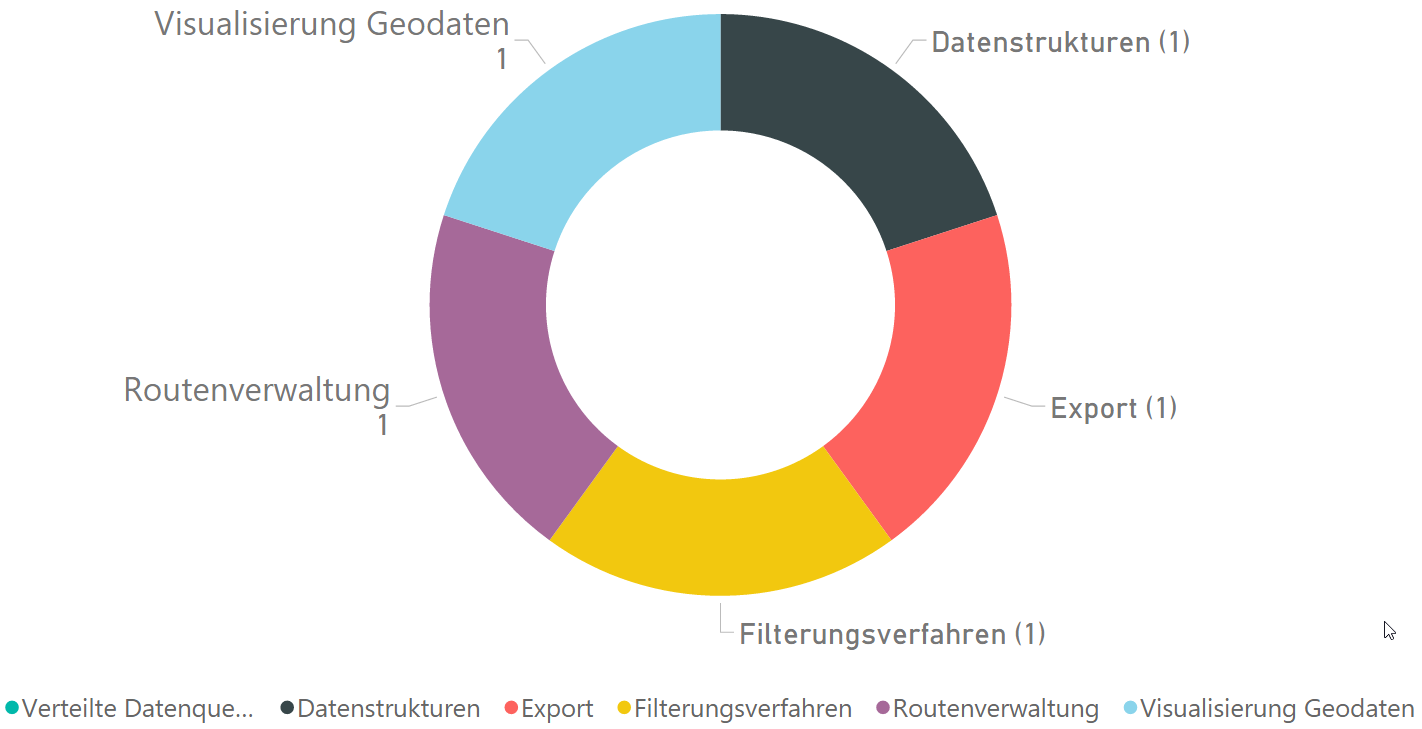
\includegraphics[width=1\linewidth]{img/Interviews/ProblemeInterview3}
\caption[Probleme in Interview III]{übersicht der genannten Probleme in Interview III (Quelle: eigene Ausarbeitung)}
\label{fig:ProblemeInterview3}
\end{figure}


\subsection*{Gemeinsamkeiten}
\label{subsubsec:Ergebnisse der Interviews:gemeinsamkeiten}
Abstrakt gesprochen unterscheiden sich die Workflows in ihren Grundzügen nicht deutlich von einander (siehe Abb.: \ref{fig:abstrakterWorkflowPlannung} - \nameref{fig:abstrakterWorkflowPlannung}). 
Es besteht eine Grundmenge von Daten (beispielsweise Kunden\_innen oder Stammdaten). 
Aus dieser Grundmenge wird mit Hilfe von Filterungs- und/oder Anreicherungsschritten die Teilmenge der relevanten Daten gebildet, was wiederum beliebig oft wiederholt wird (jeweils für jedes Entscheidungskriterium).
Nachdem die Teilmenge der relevanten Daten den Anforderungen des Szenarios entspricht, wird mit der Auswahl der einzelnen Elemente fortgefahren.
Die Menge dieser gewählten Elemente bilden schlussendlich die getroffene Auswahl für die Planung.\\
\\
Bei diese Schilderung handelt es sich nur um den kleinsten gemeinsamen Nenner der geführten Interviews.
Die Unterschiede liegen dabei in den Details, wie beispielsweise die Auswahl für die Teilmenge der relevanten Daten gebildet wird.
Speziell die Probleme, die in den jeweiligen Details auftreten werden im folgenden Abschnitt genauer erläutert.

\begin{figure}[h]
	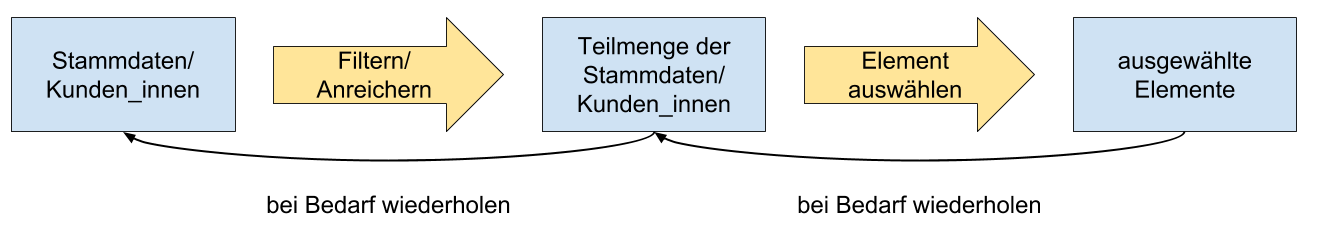
\includegraphics[width=\linewidth]{img/analyse/abstrakterWorkflowPlannung}
	\caption[abstrakter Planungsworkflow]{abstraktes Model des Planungsworkflows (Quelle: eigene Ausarbeitung)}
	\label{fig:abstrakterWorkflowPlannung}
\end{figure}

Mithilfe der Interviews wurden zwei weitere Phasen identifiziert, welche für die Praxis von hoher Relevanz sind und im vorhergehenden Kapitel noch nicht beachtet wurden.
Dabei handelt es sich zum einen um die Unterstützung während der Durchführung der Außendiensttätigkeit und zum anderen um die Aufbereitung der Daten nach der Außendiensttätigkeit.

\subsection*{Analyse}
\label{AnalyseInterviews}
Alle in den \nameref{chap:analyse:sec:interviews} besprochenen Workflows haben an gewissen Stellen Verbesserungspotential. 
Das Ziel dieses Abschnitts besteht darin die genannten Probleme und Wünsche (beziehungsweise die Ursachen der Wünsche) in Kategorien zusammenzufassen.
Basierend auf dieser Kategorisierung soll später das Konzept für den Prototypen evaluiert werden.


\def\arraystretch{1.5} %  1 is the default, change whatever you need
\begin{table}[h!]
	\begin{tabular}{|p{5cm}|p{2,25cm}|p{2,25cm}|p{2,25cm}|}
		\hline  
		& \ctab \nameref{anhang:interview1} 
		& \ctab \nameref{anhang:interview2} 
		& \ctab \nameref{anhang:interview3} \\ 
		\hline 
		\nameref{p1}
		& \ctab X
		& \ctab X
		& \ctab  \\ 
		\hline 
		\nameref{p2}
		& \ctab  X
		& \ctab X
		& \ctab  \\ 
		
		\hline 
		\nameref{p3}
		& \ctab  
		& \ctab X
		& \ctab X \\ 
		\hline 
		\nameref{p4}
		& \ctab 
		& \ctab  X
		& \ctab X \\ 
		\hline 
		\nameref{p5}
		& \ctab 
		& \ctab (indirekt)
		& \ctab X \\ 
		\hline 
		\nameref{p6}
		& \ctab X
		& \ctab X
		& \ctab  \\ 
		\hline 
	
	\end{tabular} 
	\caption[Zusammenfassung der Probleme]{Übersicht der zusammengefassten Probleme der einzelnen Interviews (Quelle: eigene Ausarbeitung)}
	\label{tab:problemeInterviews}
\end{table}


\subsubsection*{Systembruch}
\label{interviewsAnalyseSystembruch}
Damit ist gemeint das parallel zum bestehenden System zusätzliche Drittsoftware oder gar andere Medien eingesetzt werden.
Diese Maßnahme sind, laut den geführten Interviews, auf den Grund zurückzuführen, dass jenes bestehende System entweder nicht über die benötigte Funktionalität verfügt
\footnote{
	Diese Meinung stammt aus der Sicht des Personals. 
	Ein weiteres denkbares Szenario ist, das die Funktionalität zwar gegeben ist, allerdings das Personal nicht darüber informiert beziehungsweise geschult wurde.
	} 
oder nur umständlich/aufwendig zu bedienen ist.
Dabei können solche Systembrüche zu den diversen Problemen führen. 
Mögliche Probleme können im Datenschutz
\footnote{
	Beispielsweise Weitergabe von Kunden/Patientendaten an Dritte.
	}
	, der unautorisierten Weitergabe von Firmengeheimnissen oder schlichtweg in Brüchen des Informationsmanagement liegen.  
Bei den durchgeführten Interviews wurden folgende drei Szenarien mit Systembrüchen identifiziert:

\paragraph{Termine und Kalender}
Auf Grund der fehlenden Funktionalität Termine im bestehenden System zu verwalten wird in \nameref{anhang:interview1} beschrieben das die Terminplanung mithilfe eines Taschenkalenders bewältigt wird. 
In \nameref{anhang:interview3} wird eine Kombination aus einem privaten Kalender in Microsoft Outlook und einem Taschenkalender verwendet. 
Bei beiden Interviews besteht das Problem das die Termine nicht für Dritte (Beispiel: Urlaubsvertretungen, etc.) einsichtig sind.

\paragraph{Routenberechnung}
Um eine Routenberechnung zu den ausgewählten Partnerunternehmen zu optimieren wird, laut \nameref{anhang:interview2} und \nameref{anhang:interview3}, regelmäßig auf Google Maps zurückgegriffen. 
Für diesen Zweck müssen die Kontaktdaten entweder umständlich kopiert oder von Hand übertragen werden.

\paragraph{Export der Daten für den Außendienst}
Ein weiterer Punkt für die Verwendung von Drittsoftware liegt in der Aufbereitung der Informationen für den Außendienst.
Nachdem eine Route geplant wurde müssen wichtige Informationen, wie Beispielsweise Verkaufzahlen und ähnliches auf Papier vorliegen. 
Für diesen Zweck werden entweder, wie in \nameref{anhang:interview2} genannt, die wichtigsten Informationen auf Post It`s übertragen oder, wie in \nameref{anhang:interview3} beschrieben, von Hand mittels kopieren und einfügen in ein Textverarbeitungsprogramme übertragen und anschließend gedruckt.

\subsubsection*{Datenstrukturen}
\label{interviewsAnalyseDatenstrukturen}
Während im letzten Abschnitt auf die bestehenden Systembrüche eingegangen wurde, liegt der Schwerpunkt hier auf den unzureichenden Datenstrukturen und weniger auf der Funktionalität der bestehenden Systeme. 
Dabei ist zu berücksichtigen, dass die richtige Datenstruktur eine Grundlage für die Implementierung von Funktionalitäten darstellt. 
Bei der Analyse der Interviews sind dabei folgende Nennungen hervorgetreten:

\paragraph{Termine}
Sowohl in \nameref{anhang:interview1} wie auch in \nameref{anhang:interview3} ist es möglich Termine beziehungsweise Datums im System zu hinterlegen. 
Allerdings handelt es sich bei den Datumsfeld, bei beiden System, ausschließlich um Textfelder. 
Das bedeutet das man zwar das Datum angeben kann allerdings das System sehr eingeschränkt ist bei der Interaktion mit diesen Werten. 
Somit lassen sich keine Operationen wie zum Beispiel wiederkehrende Termine erstellen (siehe \nameref{anhang:interview3}) und hat somit nur einen stark eingeschränkten Mehrwert.


\paragraph{Kundenspezifische Meta-Daten}
Der letzte Punkt behandelt die fehlenden Datenstrukturen von kundenspezifischen Meta-Daten.
Dieser Begriff wurde im Zuge der Interviews vom Autor geprägt und bezeichnet Daten und Informationen über Kunden, die nicht zu den klassischen Firmendaten, wie Beispielsweise Umsatzzahlen zählen. 
Vielmehr haben diese Informationen den Charakter von firmeninternen Notizen, wie sie auch in den meisten System aktuell gehandhabt werden.
Ein Beispiel für diese Daten wären zum Beispiel die persönlichen Interessen/Abneigung, Smalltalk-Themen und produktiv Zeiten\footnote{Beispiel: ...ist Frühaufsteher, ...Abschlüsse lassen sich am besten am Abend machen, etc.} der Kunden\_innen. 
Wie in \nameref{anhang:interview2} \nameref{anhang:interview3} festgestellt wurde, sind diese Daten für die Personen in der Planung ein hilfreiches Werkzeug. 
Leider ist im besten Fall bei Kundenkontakten ein allgemeines Notizfeld. 
Ähnlich wie bei den Terminen ist es schwierig diese Daten sinnvoll zu verwenden solang sie nur als reiner Text vorliegen.

\subsubsection*{Routenverwaltung}
\label{interviewsAnalyseRoutenverwaltung}
Das Endprodukt einer Außendienstplanung stellt eine fertig gestellte Route da mit allen Daten und Informationen die der Außendienstmitarbeiter für die Durchführung benötigt.
Leider ist in keinen der durchgeführten Interviews aktuell eine solche Funktion gegeben oder angedacht.
Im Moment werden Aspekte der Routenverwaltung bei allen drei Interview angegeben.
Dabei handelt es sich um die Erstellung, die Bearbeitung und das Exportieren für den Außendiensteinsatz (siehe \nameref{anhang:interview1}, \nameref{anhang:interview2} und \nameref{anhang:interview3}). 

\subsubsection*{Filterungsverfahren}
\label{interviewsAnalyseFilterungsverfahren}
Den ersten Schritt der Planung stellt das Filtern nach relevanten Datensätzen da.
Aktuell geschieht dies, im besten Fall, durch das definieren von verschiedenen Filtereinstellungen (Beispielsweise in pery).
Umständlich wird es, wenn die benötigten Daten auf verschiedenen nicht mit einander verbundenen Systemen verteilt sind (siehe Abschnitt \nameref{interviewsAnalyseSystembruch}). 
Diese Verteilung hat in der Praxis zur Folge, dass Zwischenergebnisse notiert und händisch miteinander verglichen werden müssen.
Was wiederum zum einen umständlich und zum anderen Fehleranfällig ist, in Hinsicht darauf, dass Daten übersehen werden können (siehe \nameref{anhang:interview2} und \nameref{anhang:interview3}).


\subsubsection*{Übersicht Standorte}
\label{interviewsAnalyseStandorte}
Bei allen Workflows spielt der Standort, der einzelnen Kunden, eine entscheidende Rolle bei der Planung.
In den meisten Systemen ist bei jedem Kontakt eine Adresse hinterlegt und wird in Form einer Textausgabe angezeigt.
Da in allen drei Interviews die fehlende Übersicht der jeweiligen Standorte am häufigsten angegeben wurde, sollte man die Ursachen genauer betrachten. 
Die Nennungen wurden dabei in folgende zwei Kategorien eingeteilt:

\paragraph{Übersicht der Standorte: in der Planung}
Nach der Filterung der Datensätze werden die Informationen meist in Tabellenform angezeigt.
Dabei ist jeder Kunde inklusive seiner Adresse in einer Zeile aufgeführt.
Bei keinen der Interviews wurde angegeben das außer der Adresse weitere geografische Informationen, wie beispielsweise Distanzen oder ähnliches, verfügbar sind.
Der einzige Weg eine Reihung durchzuführen basiert entweder auf der Postleitzahl
\footnote{
	numerisch auf- beziehungsweise absteigend
	} 
(siehe \nameref{anhang:interview2}) oder auf dem Namen der Stadt
\footnote{
	alphabetisch auf- beziehungsweise absteigend
	}. 
Allerdings ist der Mehrwert einer Reihung oder Filterung nach harten Grenzen (Postleitzahlen oder Stadtnamen) oft nicht zielführend, da der geografische Kontext verloren geht.
Dies wird an folgenden Beispiel deutlicher (siehe Abb. \ref{fig:HarteGrenzen} -  \nameref{fig:HarteGrenzen}). 
Angenommen es gibt zwei Kunden\_innen die eine Distanz von knapp 300 Metern trennt. 
Da sie beide durch eine Stadtgrenze getrennt sind werden sie bei der Sortierung an unterschiedlichen Stellen aufgelistet.
Dabei gehen relevante Informationen wie zum Beispiel ein Standort der 300 Meter in der nächsten Stadt liegt schlichtweg verloren (siehe \nameref{anhang:interview1} und \nameref{anhang:interview2}). 
 
\begin{figure}[h]
\centering
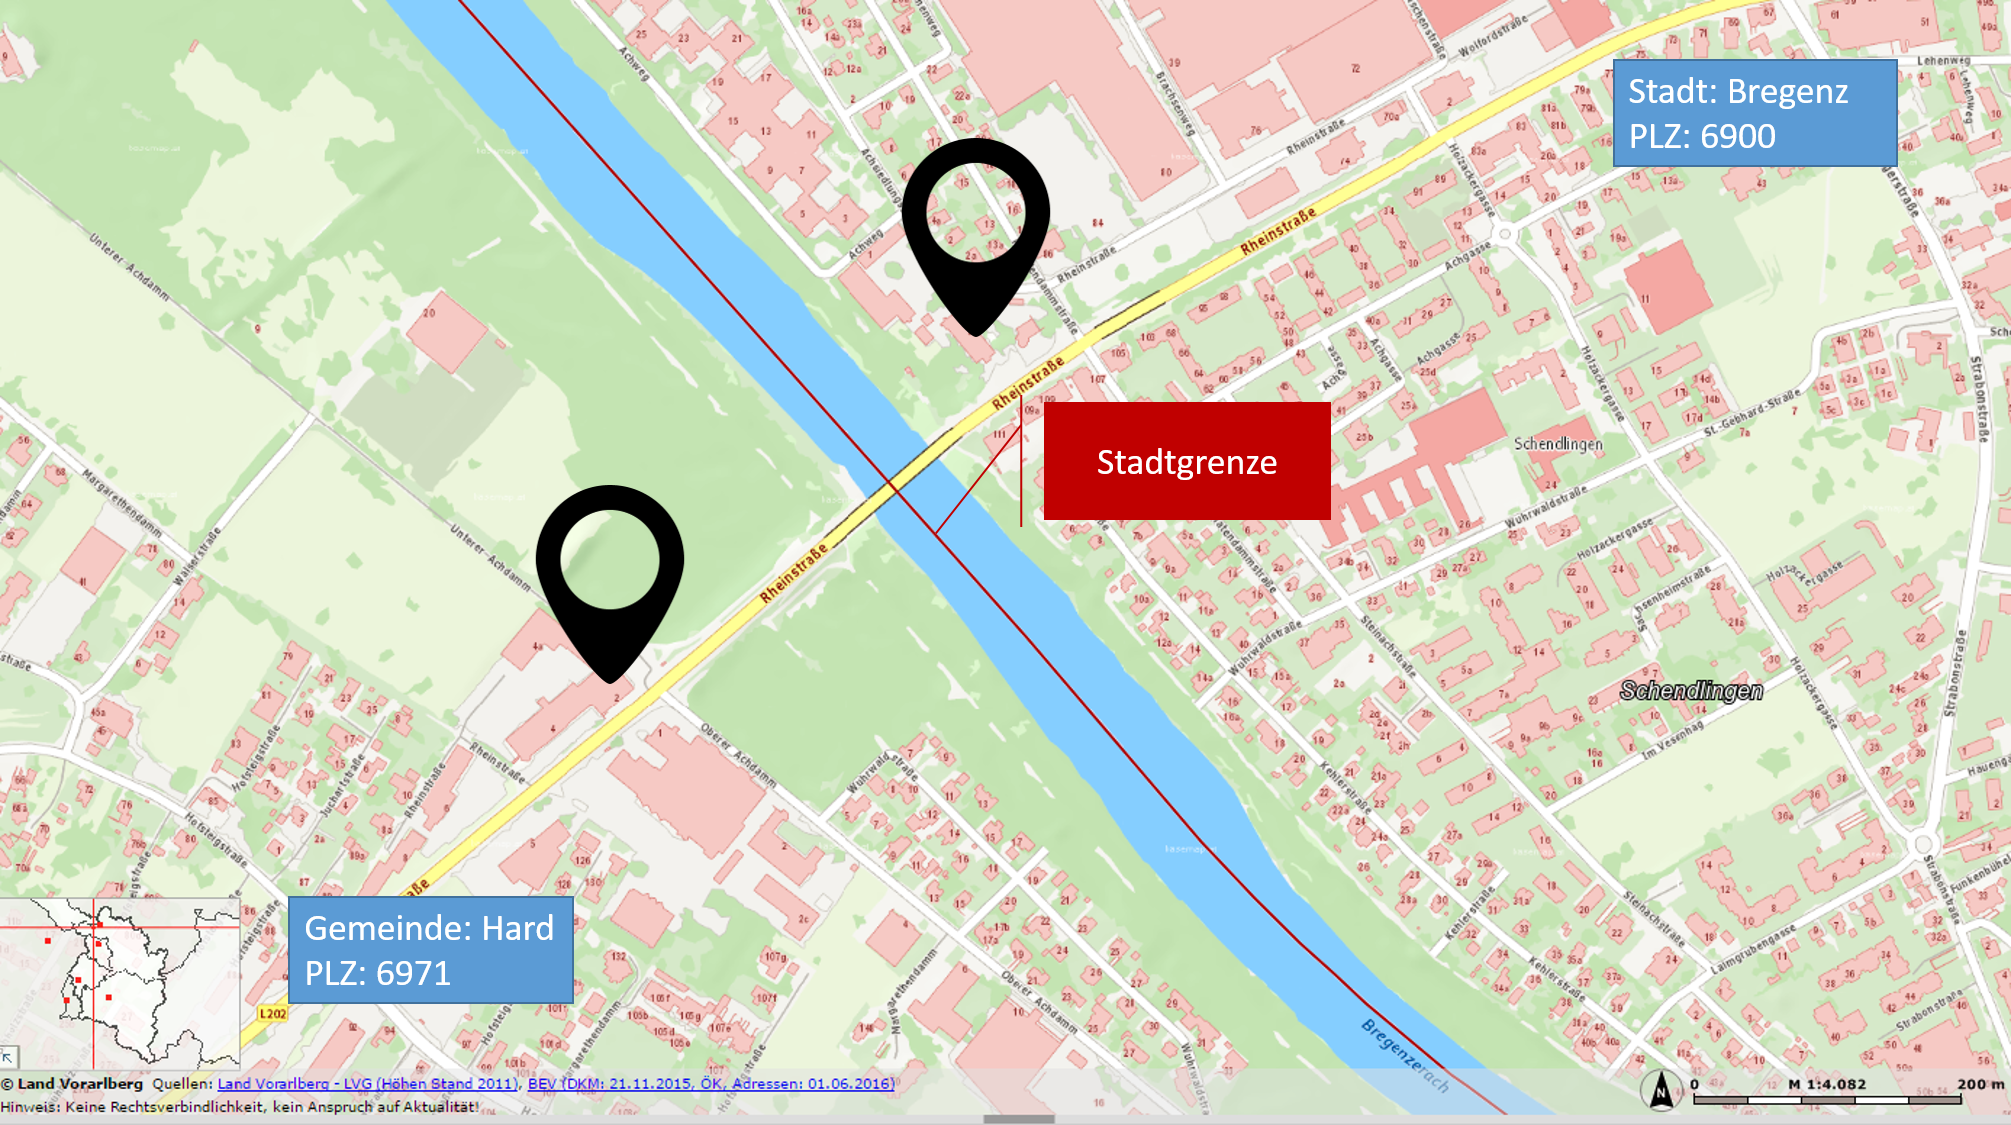
\includegraphics[width=1\linewidth]{img/Interviews/HarteGrenzen}
\caption[Probleme mit harten Grenzen]{Problem bei der Filterung oder Sortierung auf Basis von Ortsgrenzen und/oder Postleitzahlen (Quelle: eigene Ausarbeitung | Daten und Kartenmaterial: http://vogis.cnv.at/)}
\label{fig:HarteGrenzen}
\end{figure}

Die Grenze der zumutbaren Übersicht wird erreicht, wenn geografische Informationen mit weiteren Faktoren, wie Kundendaten, in Kontext gesetzt werden sollen oder. 
Dies wird aktuell in Zwischenschritten\footnote{Dabei ist die Anzahl der Zwischenschritte von der Anzahl der benötigten Faktoren abhängig} gelöst und ist zum einen Fehleranfällig und zum anderen Zeitaufwendig (siehe \nameref{anhang:interview2}).

\paragraph{Übersicht der Standorte: in der Durchführung}
Ähnlich wie bei der Planung, wurden auch bei der Durchführung des Außendiensteinsatzes Defizite bei der Übersichtlichkeit der Standorte festgestellt. 
Dies tritt vor allem dann auf wenn durch Änderungen spontan reagiert werden muss.
Dies sind meisten Einschübe oder Änderungen von Termin während des Einsatzes (siehe \nameref{anhang:interview2}). 
In solchen fällen muss zugig ein Ersatz gefunden werden
Dafür bieten sich meist Kunden in der nähe an.
/ fehlende Ortskenntnisse - Vertretung (I1) \\
/ Termine einschieben (I1)\\
/ Welcher Kunde ist in der nähe (I2)\\


\begin{comment}
\paragraph*{1. Daten sind auf verschiedene Medien und Systeme verteilt}
\label{p1}
Bei zwei der durchgeführten Interviews ist aufgefallen, das die benötigten Daten für die Planung auf unterschiedliche Systeme verteilt sind.
Dies geht soweit, das sogar Medienbrüche (Papierkalender - siehe: \nameref{anhang:interview1}) stattfinden.
Bei dem Beispiel, handelt es sich um wiederkehrende Termine, die leicht im Kalender übersehen werden können. Durch solch ein versäumen, entsteht ein Umplanungsverfahren, welches Zeit- und Ressourcen aufwendiges ist.\\
\\
Im Gespräch stellt sich heraus, dass es für diese Patchwork-Konstruktion zwei Ursachen gibt.
Diese liegen zum einen darin, dass den Anwender\_innen nicht der gesamte Funktionsumfang ihrer Lösung bekannt ist, sowie aus Gewohnheit und/oder persönlicher Vorliebe andere Werkzeuge präferiert werden.
Zum anderen, stellen die vorhandenen Organisationswerkzeuge nicht denn benötigten Funktionsumfang zur Verfügung, woraufhin dritte Systeme oder Medien als Unterstützung evaluiert und eingesetzt werden. 

\paragraph*{2. Filterung von Kunden auf Basis von geografischen Grenzen (Stadt, Land, etc.)}
\label{p2}
\ideas{
	\begin{itemize}
		\item Persönliche Ortskenntnisse notwendig
		\item - Probleme bei Vertretungen von anderen Einzugsgebieten
		\item Filterung auf Basis von PLZ
		\item Zwei Kunden können nebeneinander liegen (aneinander liegenden Stadträndern), werden aber auf Grund von harten Grenzen ausgefiltert.
	\end{itemize}
}

\paragraph*{3. Umständliche/mehrfache Filterungsschritte}
\label{p3}
\ideas{
	\begin{itemize}
		\item Teilweise müssen erst Zwischenabfragen getätigt werden und die Ergebnisse notiert werden um sie anschließend im nächsten Filter wieder einzutragen - Filterworkflow 
		\item Teilweise Filtern über verschiedene Systeme/Software hinweg mit Copy and Paste
	\end{itemize}
}

\paragraph*{4. Keine Möglichkeit Routen zu verwalten }
\label{p4}
\ideas{
	\begin{itemize}
		\item wiederholende Routen mit minimalen oder keinen geänderten Parametern
		\item ausgewählte Kunden werden auf PostIts übertragen (Interview II) - Aufwendig und Fehleranfällig
	\end{itemize}
}

\paragraph*{5. Fehlende Visualisierung von Distanzen}
\label{p5}


\paragraph*{6. Fehlende Überblick welcher Kunde ist in der Nähe ist}
\label{p6}
\ideas{
	\begin{itemize}
		\item Speziell bei spontanen Änderungen im Außendienst, Termin verschiebt sich oder fällt aus.
	\end{itemize}
}

\paragraph*{7. Fehlende Möglichkeiten für kundenspezifischen Metadaten}
\label{p7}
\ideas{
	\begin{itemize}
		\item Laut allen drei Interview sind Hinterlegungen für interne Anmerkungen über Kunden bzw. Ansprechperson sehr essentiell und auch in der Planung berücksichtigt
		\item Werden oft nur als Notizfelder von Programmen angeboten.
		\item Evtl. nicht relevant bzw. als zusätzliche Information 
	\end{itemize}
}

\paragraph*{8. Umständliche Exportmöglichkeiten von Kunden-/Stammdaten}
\label{p8}
\ideas{
	\begin{itemize}
		\item Stammdatenblätter sind für die Durchführung wichtig
		\item Werden vor der Tour händisch exportiert und ausgedruckt
	\end{itemize}
}
\end{comment}




\section{Persona}
\label{persona}
\ideas{Entwicklung der Persona beschreiben, evtl noch in die Analyse packen}

\section{Konzept}
\label{chap:entwicklung:sec:konzept}

\ideas{Konzept für die ersten Entwürfe aus den Ergebnisse der Analyse mergen}

\paragraph{Eigenschaften der Routenverwaltung}

Es soll Grundsätzlich möglich sein Routen im System zu erfassen und diese zu bearbeiten (siehe \nameref{anhang:interview1}).
Desweiteren sollte sich die Reihung der Route ändern lassen um spontan auf Verkehrsstaus oder Terminverschiebungen reagieren zu können (siehe \nameref{anhang:interview2}).
Zusätzlich dazu sollten sich die Route sowie die kunderelevanten Daten einfach exportieren und ausdrucken lassen (siehe \nameref{anhang:interview2} und \nameref{anhang:interview3}). 
Abschließend kann, auf Basis der Routenverwaltung, ein erleichterter Zugang zu der Dokumentation des Außendiensteinsatzes geschaffen werden (siehe \nameref{anhang:interview3})

\section{Design-Entwurf}
\label{chap:entwicklung:sec:design_entwurf}

merken der Kartenposition

\ideas{Dokumentation des Entwicklungsprozesse vom \nameref{chap:entwicklung:sec:konzept} zum \nameref{chap:entwicklung:sec:design_entwurf:sub:mockUps} \\
	\\
	Entwicklung nach "'user centered design"
	\\
	UI-Design Studie: 
	\begin{itemize}
		\item Welche Darstellung unterstützt den/die Anwender\_in am ehesten
		\item Map- vs. List-View (evtl. weitere Darstellungsmöglichkeiten)
		\item Sinnvolle Visualisierung von Prioritäten 
		\item Auswahl basierte Darstellung für UI 
	\end{itemize}}

\subsection{Ziele der Gestaltung}
\label{chap:entwicklung:sec:design_entwurf:subs:ziele_der_gestaltung}

\ideas{Definition auf welche Ziele hingearbeitet werden soll - Einfluss der Erkenntnisse aus Abschnitt: \nameref{chap:entwicklung:sec:konzept}}

\begin{comment}
Um die Ziele der Gestaltung definieren zu können muss zuerst analysiert werden, wie die Zielgruppe ihre Wünsche und Erwartungen an die Applikation definiert.\\

\subsubsection*{Ziel: Übersichtlichkeit}
\label{subsub:ziel_uebersichtlichkeit}
Eine klare und aufgeräumte Oberfläche ist notwendig, um die Unterstützung der Benutzer zu maximieren. 
Dazu zählt das Aufteilen der Inhalte in sinnvolle und logische Gruppen unter der Berücksichtigung der Arbeitsabläufe.


\subsubsection*{Ziel: Vertraute Umgebung}
\label{subsub:ziel_vertraute_umgebung}
Durch das Erzeugen einer vertrauten Umgebung sollen die Nutzer bekannte Elemente ihrer Plattform in der Applikation wiedererkennen.
Dadurch sollen die Einarbeitungszeiten in die Applikation minimiert, sowie der Wiedererkennungswert von plattformtypischen Elementen wie beispielsweise die Navigation durch das Programm, maximiert werden.
Es wird versucht, dass die Benutzer jeder Zeit das Gefühl haben, dass sie das Programm vollständig kontrollieren.
Dadurch soll den Nutzern die Angst genommen werden "`etwas falsches zu machen"'.
Für die Realisierung dieses Zieles muss sich die Applikation an dem Standartverhalten der jeweiligen Plattform orientieren.
\newpage
\end{comment}


\subsection{Mock-Ups - Prototyp Entwicklung}
\label{chap:entwicklung:sec:design_entwurf:sub:mockUps}

\ideas{Dokumentation der Entstehung sowie Überlegungen des ersten Prototypen}

\begin{comment}
Um schon in einem frühen Stadium des Entwicklungsprozesses\\ Rückmeldungen über die Bedienbarkeit des Programmes zu erhalten, empfiehlt es sich, in die Entwicklung von Mock-ups zu investieren.
Unter Mock-Ups versteht man einen nicht funktionellen Prototypen. 
Dies bedeutet, dass der Prototyp nicht programmiert, sondern mit einem Bildbearbeitungsprogramm erzeugt wird.
Dabei wird für jede Ansicht ein eigener Prototyp "`gezeichnet"'. 
Anschließend werden mit Personen aus der Zielgruppe die einzelnen Szenarios der Applikation simuliert. 
Während des Testes sollen die NutzerInnen den Ablauf des Programmes, die erwarteten ihrer Ergebnis von Interaktionen sowie ihre Emotionen so detailliert wie möglich kommentieren.  
Mithilfe des Testes lässt sich feststellen, wie schlüssig die Arbeitsabläufe sind, ob die Funktionalität der Oberfläche verständlich ist und ob die Reaktionen des Programmes mit den Erwartungen der Benutzer übereinstimmen. 
Der Prozess des \texttt{Paper Prototyping} sollte nicht einmalig, sondern in Form eines iterativen Entwicklungsprozess durchgeführt werden. 
Dies bedeutet, dass auf der Basis der erhaltenen Rückmeldungen die Mock-Ups optimiert und die Test wiederholt werden.
Der Test kann als positiv betrachtet werden, wenn die Rückmeldungen der Probanden mit den zuvor definierten Design-Zielen (siehe Abschnitt: \nameref{sub:ziele_der_gestaltung}) übereinstimmen.\\
\\
Die Mock-Ups der Beispiel-Applikationen befinden sich im Anhang:  \nameref{chap:diagramme_und_bilder} unter dem Abschnitt: \nameref{sec:mock_ups}. 
\end{comment}

\newpage




\end{document}
